\documentclass[10pt, compress]{beamer}
\usetheme[titleprogressbar]{m}

\usepackage{booktabs}
\usepackage[scale=2]{ccicons}
\usepackage{minted}

\usepgfplotslibrary{dateplot}

\usemintedstyle{trac}

\title{FShark}
\titlegraphic{\includegraphics[width=\textwidth,height=.5\textheight]{fsharklogo.png}}
\subtitle{Effortless GPU Programming in F\#}
\author{Mikkel Storgaard Knudsen}
\institute{Master's Thesis presentation, University of Copenhagen}

\begin{document}

\maketitle

\begin{frame}[fragile]
\frametitle{Introduction}
The future demands more efficient computing
\pause 
not achievable by common sequential programming 

% CUDA and OpenCL exists, but is a nuisance to write, and to use in mainstream languages

% we want a way to both develop and use efficient GPU computational kernels
% within mainstream language contexts.


\begin{figure}
  \centering
 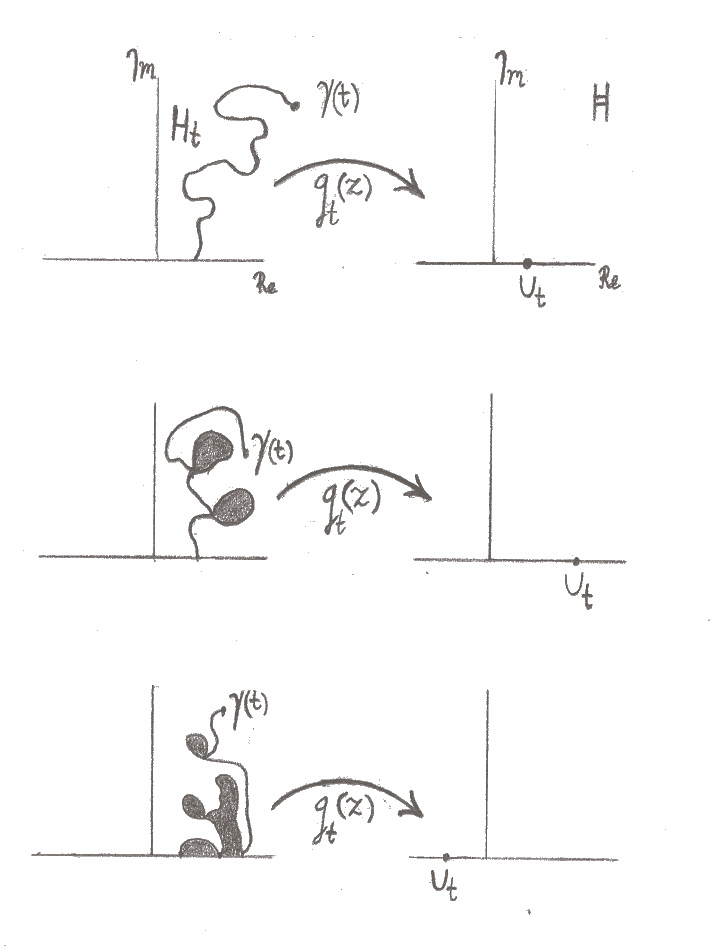
\includegraphics[width=6cm,height=6cm]{firstex.png}
\end{figure}

\end{frame}

\begin{frame}[fragile]
  \frametitle{birds eye}
  % what is the contribution of fshark
  
  %% c# computational kernel generator for futhark
  %%% short explanation of current state of futhark
  %%% use case for futhark c# code generator
  %%% show diagram of futhark compilation pipeline
  %%%% for each part, elaborate and show example

  %% language with library
  %%% explain use case
  %%% show short code example

  %% fshark transpiler and wrapping framework
  %%% explain use case
  %%% show large diagram of components, and explain individual parts
  %%%% for each part, elaborate and show example
  

\begin{figure}
  \centering
 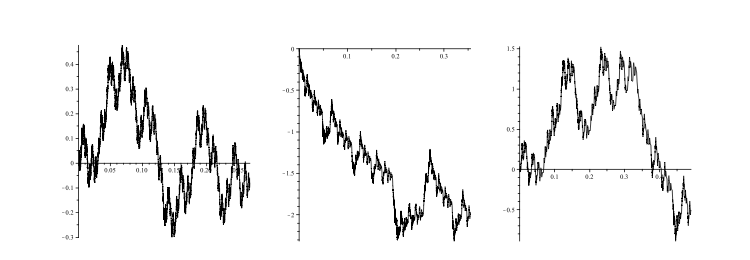
\includegraphics[width=11cm,height=4cm]{intro2.png}
\end{figure}
\tiny
source: "spacefilling curves and phases of the loewner equation", j.lind, s.rohde
\normalsize
\end{frame}

\begin{frame}[fragile]
  \frametitle{Challenging aspects of the implementation}
  % Choosing what types FShark should support, and how to implement the support
  % for these types. in particular the whole ding about arrays.

  % interoperability between F# and generated C# libraries



\begin{figure}
  \centering
 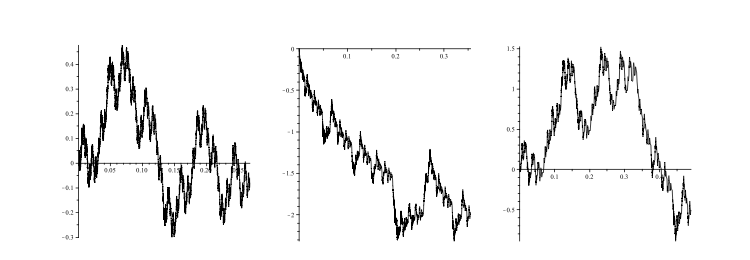
\includegraphics[width=11cm,height=4cm]{intro2.png}
\end{figure}
\tiny
source: "spacefilling curves and phases of the loewner equation", j.lind, s.rohde
\normalsize
\end{frame}

\begin{frame}[fragile]
  \frametitle{Evaluation}

  

\begin{figure}
  \centering
 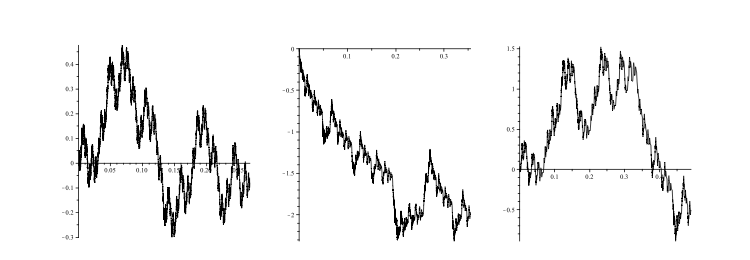
\includegraphics[width=11cm,height=4cm]{intro2.png}
\end{figure}
\tiny
source: "spacefilling curves and phases of the loewner equation", j.lind, s.rohde
\normalsize
\end{frame}

\begin{frame}[fragile]
  \frametitle{Evaluation - Testing and correctness}

  % Futhark Code Generator (does it work as a Futhark backend?)
  %% yes, based on unit tests and benchmark suite
  
  % FShark language (Can we write complex GPU benchmarks in FShark?)

  % FShark Compiler (unit tests)

\begin{figure}
  \centering
 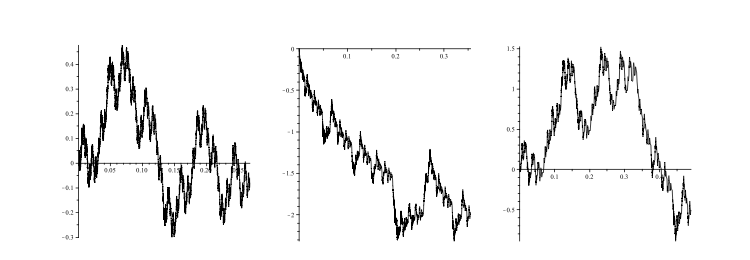
\includegraphics[width=11cm,height=4cm]{intro2.png}
\end{figure}
\tiny
source: "spacefilling curves and phases of the loewner equation", j.lind, s.rohde
\normalsize
\end{frame}


\begin{frame}[fragile]
  \frametitle{Evaluation - Performance}

  % Look at how C# OpenCL performs compared to C OpenCL
  %% Boxplot for time increase/decrease for all benchmarks

  %% plot that describes runtime increase/decrease in correlation with input size

  %%% discuss where major differences comes from

  % Look at how C# performs compared to C
  %% Very few samples;
  %% Major differences
  %% Why are these differences so large?

  % All in all quite succesful

\begin{figure}
  \centering
 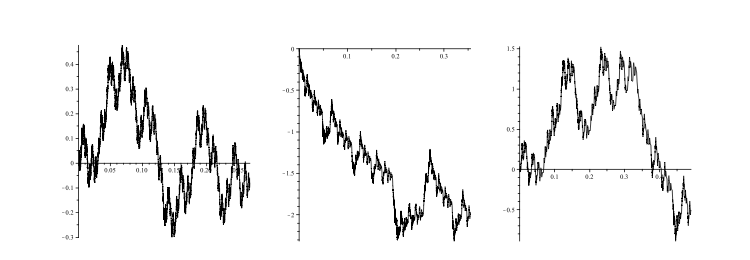
\includegraphics[width=11cm,height=4cm]{intro2.png}
\end{figure}
\tiny
source: "spacefilling curves and phases of the loewner equation", j.lind, s.rohde
\normalsize
\end{frame}

\begin{frame}[fragile]
  \frametitle{Evaluation - Usability and interoperability}

  % Live demo of writing a matrix multiplication kernel in FShark
  %% Compile using F#
  %% Use resulting C# library in a C# project
  
\begin{figure}
  \centering
 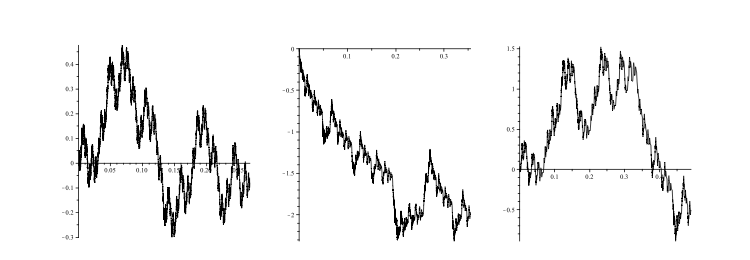
\includegraphics[width=11cm,height=4cm]{intro2.png}
\end{figure}
\tiny
source: "spacefilling curves and phases of the loewner equation", j.lind, s.rohde
\normalsize
\end{frame}


\begin{frame}[fragile]
  \frametitle{Related work}

  

\begin{figure}
  \centering
 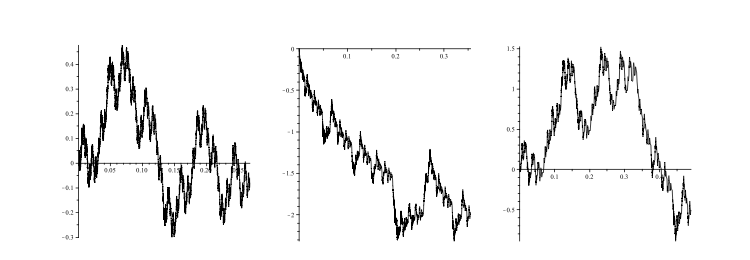
\includegraphics[width=11cm,height=4cm]{intro2.png}
\end{figure}
\tiny
source: "spacefilling curves and phases of the loewner equation", j.lind, s.rohde
\normalsize
\end{frame}

\plain{Questions?}

\end{document}